\documentclass[10pt,journal]{IEEEtran}
\usepackage[spanish]{babel}
\usepackage[T1]{fontenc}
\usepackage{amsmath}
\usepackage{float}
\usepackage{graphicx}
\usepackage{booktabs}
\usepackage{placeins}
\usepackage{xcolor}
\usepackage{listings}

\lstdefinestyle{pythonstyle}{
  language=Python,
  basicstyle=\ttfamily\small,
  keywordstyle=\color{blue!60!black}\bfseries,
  stringstyle=\color{red!50!brown},
  commentstyle=\color{gray}\itshape,
  numbers=none,
  breaklines=true,
  showstringspaces=false,
  frame=single,
  framesep=3pt,
  xleftmargin=3pt,
  xrightmargin=3pt,
  columns=flexible,
}
\lstset{style=pythonstyle}
\usepackage[pdfauthor={Jheison Martinez Bolivar},pdftitle={Clasificacion de Candidatos a Exoplaneta Kepler mediante Aprendizaje Supervisado},colorlinks,linkcolor=blue,citecolor=green,urlcolor=cyan]{hyperref}

\begin{document}

  \title{Clasificaci\'on de Candidatos a Exoplaneta Kepler mediante Aprendizaje Supervisado:\\
    Regresi\'on Log\'istica, Naive Bayes y Random Forest}

  \author{
    Jheison Martinez Bolivar\\
    \textit{Maestr\'ia en Inteligencia Artificial}\\
    \textit{Universidad de La Salle, Bogot\'a, Colombia}\\
    \texttt{jhmartinez07@unisalle.edu.co}
  }
  \maketitle
  \markboth{Universidad de La Salle --- Aprendizaje de M\'aquina. Agosto 2026}{}

  \begin{abstract}
    Este trabajo aborda un problema de clasificaci\'on supervisada multiclase sobre el cat\'alogo acumulativo \emph{Kepler Objects of Interest} (KOI) de la NASA (9\,564 registros), en el cual cada detecci\'on de tr\'ansito debe etiquetarse como \texttt{CONFIRMED}, \texttt{CANDIDATE} o \texttt{FALSE POSITIVE}. Sobre este cat\'alogo se aplic\'o un criterio expl\'icito de auditor\'ia de variables, excluyendo las columnas \texttt{koi\_score} y \texttt{koi\_pdisposition} por constituir, en la pr\'actica, la respuesta ya calculada por el pipeline autom\'atico de vetting de la NASA. Con un conjunto final de 17 variables f\'isicas del tr\'ansito y de la estrella, y tras un preprocesamiento con partici\'on estratificada (80\,\%/20\,\%) y escalado est\'andar, se compararon tres modelos: Regresi\'on Log\'istica multinomial, Naive Bayes Gaussiano y Random Forest. Random Forest obtuvo el mejor desempe\~no ($Accuracy=0.8946$, $F1_{ponderado}=0.8942$), seguido de Regresi\'on Log\'istica ($Accuracy=0.8245$) y Naive Bayes ($Accuracy=0.7087$). El an\'alisis por clase revela que la brecha entre modelos se concentra en distinguir \texttt{CANDIDATE} de \texttt{CONFIRMED} —clases con mediciones muy similares—, mientras que Regresi\'on Log\'istica y Random Forest identifican la clase \texttt{FALSE POSITIVE} con precisi\'on y recall superiores a 0.98 (Naive Bayes tambi\'en la identifica bien, aunque con un recall algo menor, de 0.92). El cuaderno con la implementaci\'on completa se encuentra disponible en Google Colab: \url{https://colab.research.google.com/drive/1CwdZLlmRgbdxrQh-_9fcUeKQ9C-Nceyg?usp=sharing}.
  \end{abstract}

  \section{Introducci\'on}

  \IEEEPARstart{L}{a} misi\'on espacial Kepler de la NASA detecta exoplanetas mediante el \emph{m\'etodo de tr\'ansito}: monitorea el brillo de cientos de miles de estrellas en b\'usqueda de ca\'idas peri\'odicas de luminosidad, producidas cuando un planeta cruza por delante de su estrella anfitriona \cite{borucki2010}. Sin embargo, no toda ca\'ida de brillo corresponde a un planeta real: sistemas binarios eclipsantes, tr\'ansitos de fondo o artefactos instrumentales generan se\~nales indistinguibles a primera vista. Por esta raz\'on, cada detecci\'on —denominada \emph{Kepler Object of Interest} (KOI)— recibe un veredicto (\texttt{koi\_disposition}) tras un proceso de verificaci\'on: \texttt{CONFIRMED} (planeta confirmado), \texttt{CANDIDATE} (a\'un no confirmado) o \texttt{FALSE POSITIVE} (descartado) \cite{thompson2018}.

  Ante el volumen de detecciones que genera la misi\'on, la verificaci\'on manual exhaustiva no es escalable. La propia NASA aborda esto con el \emph{Robovetter}, un pipeline autom\'atico de reglas heur\'isticas que produce el cat\'alogo DR25 utilizado en este trabajo \cite{thompson2018}; en paralelo, la comunidad astron\'omica ha explorado clasificadores de aprendizaje autom\'atico supervisado como alternativa o complemento a ese tipo de heur\'isticas. Este trabajo, desarrollado en el marco de la Maestr\'ia en Inteligencia Artificial de la Universidad de La Salle y como continuaci\'on de una actividad previa sobre regresi\'on de excentricidad orbital, aborda precisamente ese problema: clasificar autom\'aticamente cada KOI a partir de las caracter\'isticas medibles de su se\~nal de tr\'ansito y de su estrella anfitriona.

  Se comparan tres algoritmos supervisados de naturaleza distinta: \textbf{Regresi\'on Log\'istica} (modelo lineal, usado como referencia base) \cite{cox1958}, \textbf{Naive Bayes} (modelo probabil\'istico generativo) \cite{rish2001}, y \textbf{Random Forest} (ensamble de \'arboles de decisi\'on) \cite{breiman2001}. El objetivo no es \'unicamente reportar m\'etricas agregadas, sino entender \emph{por qu\'e} un modelo supera a otro a la luz de sus supuestos estad\'isticos y de la naturaleza del problema.

  \section{Datos y Preprocesamiento}

  \subsection{Selecci\'on del Conjunto de Datos}

  La elecci\'on del dataset definitivo requiri\'o un proceso de descarte. Un primer candidato, \emph{NASA Exoplanet Archive Intelligence}, ofrec\'ia una columna booleana \texttt{habitable\_zone\_flag} como target natural. Sin embargo, al auditar su relaci\'on con las dem\'as variables se encontr\'o que \emph{todas} las columnas categ\'oricas de ese dataset —incluida \texttt{habitable\_zone\_flag}— eran en realidad reglas de binning deterministas sobre columnas num\'ericas que permanec\'ian en el propio dataset (por ejemplo, \texttt{star\_type} coincid\'ia exactamente con rangos fijos de \texttt{star\_temp\_k}, y \texttt{multi\_planet\_system} era id\'entica a la condici\'on \texttt{n\_planets > 1} en el 100\,\% de los casos). Entrenar un clasificador sobre esas variables habr\'ia significado que el modelo aprendiera a repetir una f\'ormula ya calculada, no un patr\'on real. Este hallazgo motiv\'o migrar al cat\'alogo \textbf{Kepler Objects of Interest (KOI)} \cite{kaggle_koi_dataset}, cuyo target (\texttt{koi\_disposition}) corresponde a un veredicto de verificaci\'on humana/autom\'atica genuino y ampliamente documentado en la literatura astron\'omica \cite{thompson2018}.

  \subsection{An\'alisis Exploratorio y Balance de Clases}

  El dataset KOI contiene 9\,564 registros y 50 columnas, cuyo significado f\'isico est\'a documentado oficialmente por el NASA Exoplanet Archive \cite{nasa_koi_columns_2026}. La variable objetivo \texttt{koi\_disposition} presenta tres clases con un desbalance moderado: \texttt{FALSE POSITIVE} (52.52\,\%), \texttt{CONFIRMED} (23.98\,\%) y \texttt{CANDIDATE} (23.50\,\%). La Figura~\ref{fig:nulos} muestra el porcentaje de valores nulos por columna.

  \begin{figure*}[t]
    \centering
    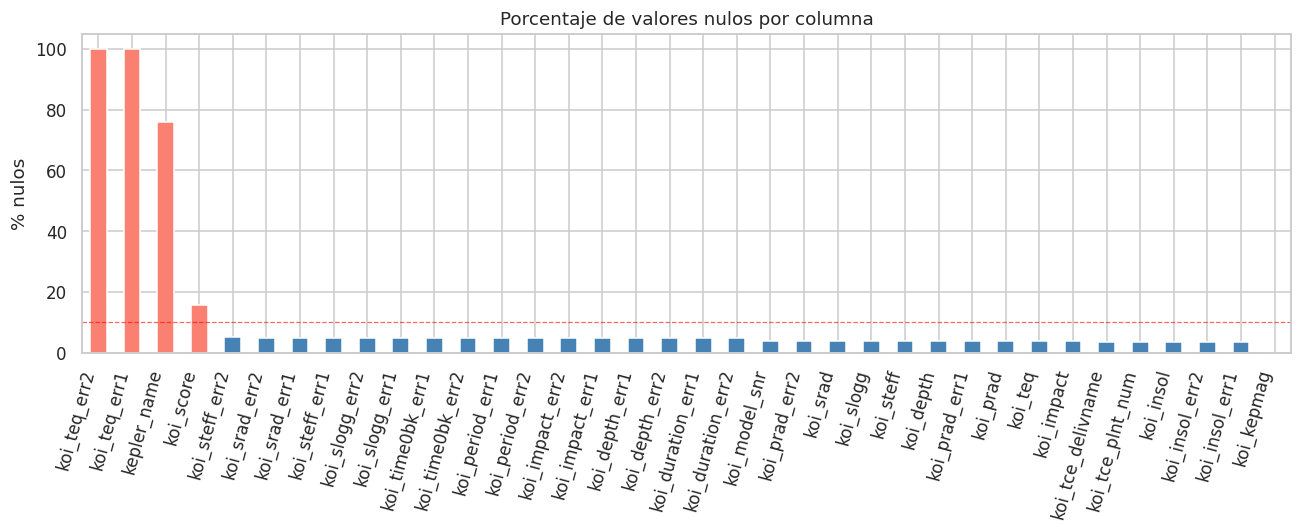
\includegraphics[width=0.85\linewidth]{assets/images/fig_nulos_koi.png}
    \caption{Porcentaje de valores nulos por variable en el cat\'alogo KOI.}
    \label{fig:nulos}
  \end{figure*}

  La Figura~\ref{fig:distcorr} visualiza esta distribuci\'on de clases junto con la matriz de correlaci\'on de Pearson entre las 13 mediciones f\'isicas continuas. Esta matriz no es solo descriptiva: revela correlaciones fuertes entre variables como \texttt{koi\_prad} y \texttt{koi\_impact} ($r=0.68$), \texttt{koi\_depth} y \texttt{koi\_model\_snr} ($r=0.58$), y \texttt{koi\_srad} con \texttt{koi\_slogg} ($r=-0.64$) —evidencia emp\'irica directa de que el supuesto de independencia condicional de Naive Bayes (Secci\'on~III-B) se viola en la pr\'actica para este conjunto de variables.

  \begin{figure*}[t]
    \centering
    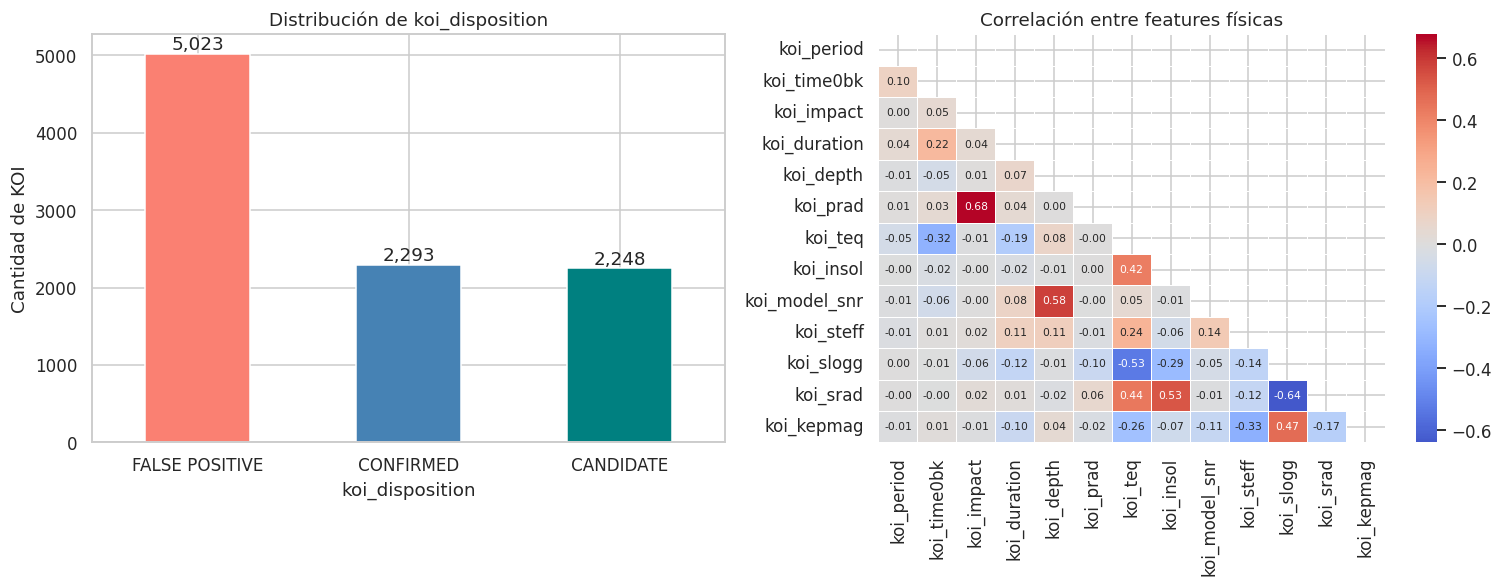
\includegraphics[width=0.85\linewidth]{assets/images/fig_dist_correlacion.png}
    \caption{Distribuci\'on de clases de \texttt{koi\_disposition} (izquierda) y correlaci\'on de Pearson entre las 13 features f\'isicas continuas (derecha).}
    \label{fig:distcorr}
  \end{figure*}

  La Figura~\ref{fig:boxplots} complementa este an\'alisis mostrando la distribuci\'on (escala logar\'itmica) de tres variables clave por clase: relaci\'on se\~nal-ruido, radio planetario y profundidad del tr\'ansito. \texttt{FALSE POSITIVE} tiende a valores m\'as dispersos y en mediana m\'as altos en las tres variables, mientras que \texttt{CANDIDATE} y \texttt{CONFIRMED} presentan distribuciones visualmente muy similares entre s\'i —evidencia visual directa de por qu\'e estas dos clases son las m\'as dif\'iciles de separar para los tres modelos (Secci\'on~\ref{sec:resultados}).

  \begin{figure*}[t]
    \centering
    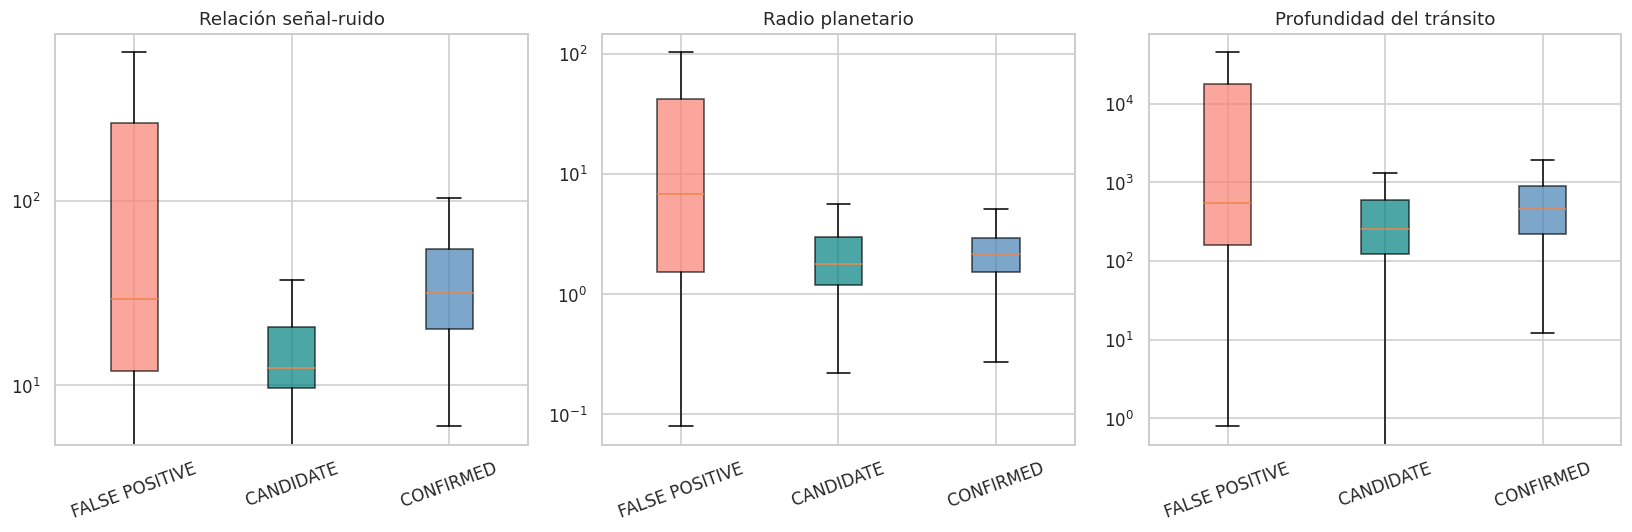
\includegraphics[width=0.85\linewidth]{assets/images/fig_boxplots_clase.png}
    \caption{Distribuci\'on (escala log) de relaci\'on se\~nal-ruido, radio planetario y profundidad del tr\'ansito, por clase de \texttt{koi\_disposition}.}
    \label{fig:boxplots}
  \end{figure*}

  \subsection{Selecci\'on de Features y Prevenci\'on de Fuga de Informaci\'on}
  \label{sec:featureselection}

  Aplicando el mismo criterio de auditor\'ia usado para descartar el primer dataset —consistente con la literatura sobre fuga de informaci\'on en aprendizaje autom\'atico \cite{kaufman2012}—, se excluyeron del conjunto de predictores tres columnas por constituir fuga de informaci\'on: \texttt{koi\_score} (la confianza que el propio pipeline autom\'atico de vetting de la NASA, el \emph{Robovetter} \cite{thompson2018}, asign\'o a cada disposici\'on final; su media es de $0.015$ para \texttt{FALSE POSITIVE} frente a $0.90$--$0.96$ para las otras dos clases, es decir, casi separa el target por s\'i sola), \texttt{koi\_pdisposition} (una disposici\'on preliminar casi id\'entica a la final) y \texttt{kepler\_name} (solo se asigna una vez confirmado el planeta). Tambi\'en se descartaron los identificadores sin valor f\'isico (\texttt{rowid}, \texttt{kepid}, \texttt{kepoi\_name}), las columnas de margen de error de medici\'on y las coordenadas celestes, para mantener el conjunto enfocado en la se\~nal observada.

  El conjunto final qued\'o compuesto por 17 variables: las cuatro banderas de vetting (\texttt{koi\_fpflag\_nt/ss/co/ec}, que al validarse emp\'iricamente no resultaron perfectamente deterministas frente al target) y trece mediciones f\'isicas del tr\'ansito y la estrella (per\'iodo orbital, tiempo de referencia del tr\'ansito, par\'ametro de impacto, duraci\'on, profundidad, radio planetario, temperatura de equilibrio, insolaci\'on, relaci\'on se\~nal-ruido del modelo, temperatura estelar, gravedad superficial, radio estelar y magnitud aparente). La definici\'on exacta de cada una de estas columnas puede consultarse en el glosario oficial del NASA Exoplanet Archive \cite{nasa_koi_columns_2026}.

  \subsection{Preprocesamiento}

  \textbf{Tratamiento de valores faltantes.} Se opt\'o por eliminar las filas con nulos en las 17 variables seleccionadas, en lugar de imputarlas, por dos razones: (i) representan solo el 3.8\,\% del dataset (364 de 9\,564 filas), una p\'erdida acotada; y (ii) al tratarse de mediciones astrof\'isicas independientes entre KOI (cada fila es una estrella/tr\'ansito distinto, sin relaci\'on temporal o secuencial entre observaciones), no existe un valor de referencia (media, mediana o similar) que se pueda asumir v\'alido para la observaci\'on faltante sin introducir un sesgo artificial ajeno a la f\'isica del sistema. Tras esta eliminaci\'on se conservaron 9\,200 de 9\,564 registros (96.2\,\%).

  \textbf{Codificaci\'on de variables.} No fue necesario un paso expl\'icito de codificaci\'on: las 17 variables predictoras finales son, o bien continuas de origen num\'erico (las 13 mediciones f\'isicas), o bien binarias ya codificadas como $0$/$1$ en el propio cat\'alogo (las cuatro banderas de vetting). La variable objetivo \texttt{koi\_disposition}, aunque categ\'orica, se dej\'o como texto (\texttt{CONFIRMED}/\texttt{CANDIDATE}/\texttt{FALSE POSITIVE}) sin codificaci\'on num\'erica adicional, ya que los tres clasificadores de \texttt{scikit-learn} utilizados aceptan etiquetas de clase en formato \texttt{string} directamente \cite{pedregosa2011}.

  \textbf{Partici\'on y escalado.} La partici\'on se realiz\'o de forma \textbf{estratificada} (80\,\%/20\,\%, $random\_state=42$) para preservar la proporci\'on original de clases en entrenamiento y prueba, dado el desbalance detectado. Las variables se estandarizaron con \texttt{StandardScaler} ($z = \frac{x-\mu}{\sigma}$) para los modelos sensibles a la escala (Regresi\'on Log\'istica, Naive Bayes); Random Forest se entren\'o sobre las variables sin escalar, dado que su criterio de partici\'on es invariante a transformaciones mon\'otonas de cada variable.

  \section{Metodolog\'ia}

  \subsection{Regresi\'on Log\'istica Multinomial}

  Este modelo, la l\'inea base del estudio, calcula para cada KOI una probabilidad de pertenecer a cada una de las 3 clases y elige la m\'as alta. Esa probabilidad se obtiene con la funci\'on \emph{softmax}, que simplemente convierte una combinaci\'on ponderada de las 17 variables en un n\'umero entre 0 y 1 por clase, de modo que las tres probabilidades sumen 1:
  \begin{equation}
    P(y=k \mid \mathbf{x}) = \frac{\exp(\mathbf{w}_k^{\top}\mathbf{x} + b_k)}{\sum_{j=1}^{K} \exp(\mathbf{w}_j^{\top}\mathbf{x} + b_j)}
    \label{eq:softmax}
  \end{equation}
  Los pesos $\mathbf{w}_k$ (uno por variable y por clase) se ajustan durante el entrenamiento para que esa probabilidad acierte lo m\'as posible en los datos observados \cite{hastie2009}. Lo importante de este modelo es que combina las variables de forma \textbf{lineal}: no puede representar que el efecto de una variable dependa del valor de otra, por lo que su desempe\~no se resiente cuando la separaci\'on entre clases requiere justamente ese tipo de combinaci\'on.

  \subsection{Naive Bayes Gaussiano}

  Este modelo invierte la pregunta: en vez de ir directo de las variables a la clase, pregunta ``si esta observaci\'on fuera de la clase $k$, \textquestiondown{}qu\'e tan probable ser\'ia ver estos valores de $x$?'' para cada clase, y con el teorema de Bayes convierte esa respuesta en la probabilidad que realmente nos interesa:
  \begin{equation}
    P(y=k \mid \mathbf{x}) \propto P(y=k) \prod_{i=1}^{n} P(x_i \mid y=k)
    \label{eq:naivebayes}
  \end{equation}
  El nombre \emph{naive} (ingenuo) viene de un supuesto fuerte: que, conocida la clase, cada una de las 17 variables se comporta de forma \textbf{independiente} de las dem\'as (por eso el producto $\prod$ en vez de una f\'ormula conjunta m\'as compleja), y que cada variable sigue una campana de Gauss dentro de cada clase. El supuesto de independencia rara vez se cumple con variables f\'isicas correlacionadas (p. ej., profundidad de tr\'ansito y relaci\'on se\~nal-ruido, Figura~\ref{fig:distcorr}), lo cual —como se discute en la Secci\'on~\ref{sec:resultados}— explica en buena medida su desempe\~no inferior \cite{rish2001}.

  \subsection{Random Forest}

  Random Forest entrena $B=100$ \'arboles de decisi\'on independientes ($n\_estimators=100$, $min\_samples\_leaf=2$), cada uno sobre una muestra distinta de los datos y usando en cada divisi\'on solo un subconjunto aleatorio de variables \cite{breiman2001}. Cada \'arbol individual puede equivocarse, pero al final se toma la clase que la mayor\'ia de los $B$ \'arboles vot\'o:
  \begin{equation}
    \hat{y} = \text{moda}\{T_1(\mathbf{x}), T_2(\mathbf{x}), \dots, T_B(\mathbf{x})\}
    \label{eq:vote}
  \end{equation}
  A diferencia de los dos modelos anteriores, cada \'arbol puede decidir una divisi\'on \emph{condicionada} al valor de otra variable (por ejemplo, ``si el radio es grande, entonces mirar la profundidad''), as\'i que Random Forest no asume independencia entre predictores ni una frontera lineal \cite{amat_rodrigo_2026}.

  \subsection{M\'etricas de Evaluaci\'on}

  Dado el desbalance de clases, no basta con mirar cu\'antas predicciones acertaron en total (\emph{accuracy}); tambi\'en se calcul\'o, por cada clase, qu\'e tan confiables (\emph{precision}) y qu\'e tan completas (\emph{recall}) fueron las predicciones, resumidas en un solo n\'umero ($F_1$) \cite{powers2011}:
  \begin{equation}
    Accuracy = \frac{\text{predicciones correctas}}{\text{total de observaciones}}
    \label{eq:acc}
  \end{equation}
  \begin{equation}
    Precision_k = \frac{TP_k}{TP_k + FP_k}, \quad
    Recall_k = \frac{TP_k}{TP_k + FN_k}
    \label{eq:precrec}
  \end{equation}
  \begin{equation}
    F1_k = 2 \cdot \frac{Precision_k \cdot Recall_k}{Precision_k + Recall_k}
    \label{eq:f1}
  \end{equation}
  En palabras simples: \emph{precision} responde ``de lo que dije que era clase $k$, \textquestiondown{}cu\'anto acert\'e?''; \emph{recall} responde ``de lo que realmente era clase $k$, \textquestiondown{}cu\'anto logr\'e detectar?''; y $F_1$ es un promedio entre ambas para no premiar un modelo bueno en una y malo en la otra.

  Adicionalmente, se ejecut\'o validaci\'on cruzada de 5 pliegues ($k$-fold CV): repetir el entrenamiento 5 veces con particiones distintas de los datos, para confirmar que el resultado no dependi\'o de un \'unico reparto de suerte entre entrenamiento y prueba \cite{pedregosa2011}.

  \section{Resultados y Discusi\'on}
  \label{sec:resultados}

  La Tabla~\ref{tab:resultados} resume las m\'etricas ponderadas de los tres modelos, y la Figura~\ref{fig:comparacion} las compara visualmente. Vale aclarar que, en un problema multiclase con promedio ponderado por soporte, \emph{Accuracy} y \emph{Recall} ponderado son matem\'aticamente id\'enticos (por eso coinciden exactamente en cada columna de la tabla); se muestran ambos por completitud y para que la fila de \emph{Precision} y $F_1$ sea comparable, no porque aporten informaci\'on independiente entre s\'i.

  \begin{table}[H]
    \caption{M\'etricas comparativas (ponderadas por soporte) en conjunto de prueba y validaci\'on cruzada}
    \label{tab:resultados}
    \centering
    \resizebox{\linewidth}{!}{%
    \begin{tabular}{lccc}
      \toprule
      \textbf{M\'etrica} & \textbf{Reg. Log\'istica} & \textbf{Naive Bayes} & \textbf{Random Forest} \\
      \midrule
      Accuracy (Test)   & 0.8245 & 0.7087 & \textbf{0.8946} \\
      Precision         & 0.8244 & 0.8615 & \textbf{0.8939} \\
      Recall            & 0.8245 & 0.7087 & \textbf{0.8946} \\
      F1-score          & 0.8218 & 0.6416 & \textbf{0.8942} \\
      Accuracy CV-5fold & $0.7983 \pm 0.0154$ & $0.7078 \pm 0.0312$ & $\mathbf{0.8752 \pm 0.0500}$ \\
      \bottomrule
    \end{tabular}%
    }
  \end{table}

  \begin{figure}[H]
    \centering
    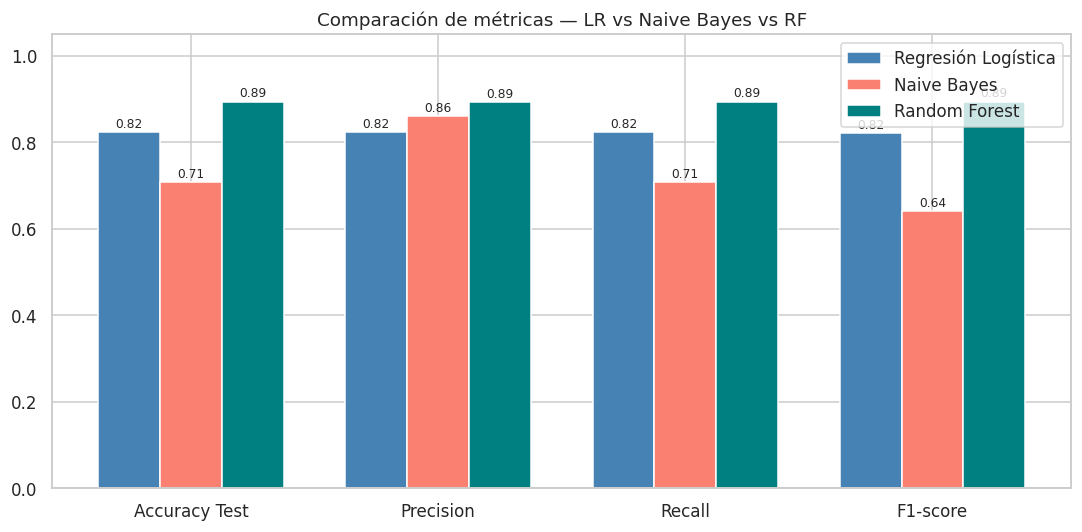
\includegraphics[width=\linewidth]{assets/images/fig_comparacion_modelos.png}
    \caption{Comparaci\'on de Accuracy, Precision, Recall y F1-score entre los tres modelos.}
    \label{fig:comparacion}
  \end{figure}

  A primera vista, la Tabla~\ref{tab:resultados} sugiere que Naive Bayes tiene una \emph{precision} razonable (0.8615), muy cercana a la de Random Forest. Esta cifra agregada es enga\~nosa: al desagregar por clase mediante el reporte de clasificaci\'on, se observa que Naive Bayes obtiene un \emph{recall} de apenas $0.01$ para la clase \texttt{CONFIRMED} —es decir, casi nunca la predice, volcando esas observaciones hacia \texttt{CANDIDATE} (cuyo recall sube artificialmente a $0.98$)—, mientras que Random Forest logra 0.81 y 0.78 de recall en \texttt{CONFIRMED} y \texttt{CANDIDATE} respectivamente, y Regresi\'on Log\'istica queda en un punto intermedio (0.75 y 0.54). Regresi\'on Log\'istica y Random Forest identifican \texttt{FALSE POSITIVE} con precisi\'on y recall superiores a 0.98; Naive Bayes tambi\'en la identifica bien, aunque su recall en esta clase (0.92) es notoriamente inferior al de los otros dos. En general, era esperable que las tres identificaran esta clase con relativa facilidad: es la mayoritaria y las cuatro banderas de vetting (\texttt{koi\_fpflag\_*}) son indicadores casi directos de descarte.

  Esta disparidad por clase, m\'as que el accuracy agregado, es el hallazgo central del experimento y admite una lectura causal ligada directamente a los supuestos de cada modelo:

  \begin{itemize}
    \item \textbf{Naive Bayes falla por su supuesto de independencia.} La Ecuaci\'on~\ref{eq:naivebayes} asume que, dada la clase, cada predictor aporta evidencia independiente de los dem\'as. En este dataset esa condici\'on se viola de forma medible (Figura~\ref{fig:distcorr}): \texttt{koi\_depth} y \texttt{koi\_model\_snr} correlacionan con $r=0.58$, y \texttt{koi\_prad} con \texttt{koi\_impact} con $r=0.68$ —un tr\'ansito m\'as profundo se traduce, en buena parte de los casos, en una se\~nal m\'as clara respecto al ruido—. Cuando la distinci\'on entre dos clases depende precisamente de c\'omo covar\'ian varias variables a la vez (y no de sus valores marginales), un modelo que ignora esa covarianza pierde la se\~nal m\'as relevante.
    \item \textbf{Una interpretaci\'on plausible es que Random Forest se beneficia de modelar interacciones no lineales.} A diferencia de la frontera lineal de la Regresi\'on Log\'istica (Ecuaci\'on~\ref{eq:softmax}) y de la independencia asumida por Naive Bayes, cada \'arbol del ensamble puede particionar el espacio de variables condicionando una divisi\'on a los valores de otra. Esta explicaci\'on es consistente con la arquitectura de cada modelo y con la brecha observada, pero este estudio no calcul\'o impor\-tancia de variables (\texttt{feature\_importances\_}) ni un an\'alisis de interacci\'on que la confirme directamente; se trata de una hip\'otesis razonada, no de un hallazgo verificado emp\'iricamente.
    \item \textbf{El accuracy global no es una m\'etrica confiable bajo desbalance de clases.} Con \texttt{FALSE POSITIVE} representando el 52.5\,\% del dataset y siendo la clase m\'as f\'acil de identificar, un modelo mediocre en las otras dos clases a\'un puede reportar un accuracy aparentemente aceptable. Esto refuerza la necesidad de reportar m\'etricas por clase (Ecuaciones~\ref{eq:precrec} y~\ref{eq:f1}) en lugar de basar las conclusiones \'unicamente en la Ecuaci\'on~\ref{eq:acc}.
  \end{itemize}

  \subsection{Ejemplo de Inferencia sobre Datos No Vistos}

  Las m\'etricas agregadas de la Tabla~\ref{tab:resultados} resumen el desempe\~no, pero conviene observar el modelo funcionando caso por caso. La Tabla~\ref{tab:inferencia} muestra la predicci\'on de los tres modelos sobre 8 KOI elegidos al azar del conjunto de prueba (\texttt{numpy.random.seed(7)}, sin selecci\'on manual posterior) —es decir, observaciones que ninguno de los tres vio durante el entrenamiento— junto con su etiqueta real.

  \begin{table}[H]
    \caption{Predicci\'on de los tres modelos sobre 8 KOI no vistos en entrenamiento (CONF.=\texttt{CONFIRMED}, CAND.=\texttt{CANDIDATE}, F.POS.=\texttt{FALSE POSITIVE})}
    \label{tab:inferencia}
    \centering
    \resizebox{\linewidth}{!}{%
    \begin{tabular}{cccc}
      \toprule
      \textbf{Real} & \textbf{Reg. Log.} & \textbf{Naive Bayes} & \textbf{R. Forest} \\
      \midrule
      CONF.   & CONF.   & \textbf{CAND.} & CONF.   \\
      F.POS.  & F.POS.  & F.POS.         & F.POS.  \\
      CAND.   & \textbf{CONF.} & CAND.   & CAND.   \\
      F.POS.  & F.POS.  & F.POS.         & F.POS.  \\
      F.POS.  & F.POS.  & F.POS.         & F.POS.  \\
      F.POS.  & F.POS.  & F.POS.         & F.POS.  \\
      CONF.   & CONF.   & \textbf{CAND.} & CONF.   \\
      CONF.   & CONF.   & \textbf{CAND.} & CONF.   \\
      \bottomrule
    \end{tabular}%
    }
  \end{table}

  Esta muestra peque\~na —y por lo tanto anecd\'otica, no estad\'isticamente representativa por s\'i sola— ilustra de forma muy concreta el patr\'on ya identificado: en los tres casos donde la etiqueta real es \texttt{CONFIRMED}, Naive Bayes predice \texttt{CANDIDATE} en los tres (su recall de $0.01$ para esta clase, reportado en la Secci\'on~\ref{sec:resultados}, no es una rareza estad\'istica sino un comportamiento sistem\'atico). Random Forest acierta las 8 de 8; Regresi\'on Log\'istica falla \'unicamente en el caso \texttt{CANDIDATE}, prediciendo \texttt{CONFIRMED} —el tipo de error opuesto al de Naive Bayes—. Las cuatro observaciones \texttt{FALSE POSITIVE} son identificadas sin excepci\'on por los tres modelos, consistente con lo discutido sobre las banderas de vetting.

  \FloatBarrier

  \section{Conclusiones}

  \begin{enumerate}
    \item \textbf{Random Forest es el modelo m\'as adecuado}: supera a Regresi\'on Log\'istica por 7 puntos de accuracy y a Naive Bayes por 18.6, con mejor desempe\~no espec\'ificamente en las dos clases dif\'iciles, \texttt{CANDIDATE} y \texttt{CONFIRMED}.
    \item \textbf{El l\'imite es tambi\'en de los datos, no solo de los modelos}: \texttt{CANDIDATE} y \texttt{CONFIRMED} se solapan fuertemente en sus 17 mediciones f\'isicas, por lo que ning\'un clasificador puede separarlas con precisi\'on perfecta usando \'unicamente estas variables.
    \item \textbf{La brecha entre modelos es consistente con sus supuestos estad\'isticos}: Naive Bayes falla por asumir independencia entre variables correlacionadas, y Regresi\'on Log\'istica por su frontera lineal. Esta lectura no se verific\'o con un an\'alisis de importancia de variables, por lo que queda como interpretaci\'on razonada y no como hallazgo confirmado.
    \item \textbf{Auditar y descartar variables con fuga de informaci\'on} (\texttt{koi\_score}, \texttt{koi\_pdisposition}) fue tan determinante para el resultado como la elecci\'on del algoritmo.
    \item \textbf{Aplicabilidad pr\'actica}: Random Forest podr\'ia usarse para priorizar qu\'e candidatos revisar primero, no para reemplazar la verificaci\'on humana.
    \item \textbf{Reproducibilidad}: cuaderno completo en Google Colab: \url{https://colab.research.google.com/drive/1CwdZLlmRgbdxrQh-_9fcUeKQ9C-Nceyg?usp=sharing}.
  \end{enumerate}

  \appendix

  \subsection{Fragmentos de C\'odigo Clave}

  El cuaderno completo y ejecutable est\'a en Google Colab (ver Conclusi\'on 6); esta secci\'on reproduce \'unicamente los fragmentos centrales para que el m\'etodo sea legible sin salir del documento.

  \textbf{Selecci\'on de features} (Secci\'on~\ref{sec:featureselection}):
  \begin{lstlisting}
TARGET = "koi_disposition"
FEATURES = [
    "koi_fpflag_nt", "koi_fpflag_ss",
    "koi_fpflag_co", "koi_fpflag_ec",
    "koi_period", "koi_time0bk",
    "koi_impact", "koi_duration",
    "koi_depth", "koi_prad", "koi_teq",
    "koi_insol", "koi_model_snr",
    "koi_steff", "koi_slogg",
    "koi_srad", "koi_kepmag",
]
  \end{lstlisting}

  \textbf{Preprocesamiento} (partici\'on estratificada y escalado):
  \begin{lstlisting}
df = df_raw[FEATURES + [TARGET]].dropna()
y, X = df[TARGET], df[FEATURES]

X_train, X_test, y_train, y_test = train_test_split(
    X, y, test_size=0.20, random_state=42, stratify=y)

scaler = StandardScaler()
X_train_sc = scaler.fit_transform(X_train)
X_test_sc = scaler.transform(X_test)
  \end{lstlisting}

  \textbf{Entrenamiento y evaluaci\'on} (Random Forest, el modelo de mejor desempe\~no; Regresi\'on Log\'istica y Naive Bayes siguen el mismo patr\'on, cambiando el estimador por \texttt{LogisticRegression} o \texttt{GaussianNB} y usando \texttt{X\_train\_sc}/\texttt{X\_test\_sc} en lugar de \texttt{X\_train}/\texttt{X\_test}):
  \begin{lstlisting}
rf = RandomForestClassifier(
    n_estimators=100, min_samples_leaf=2,
    n_jobs=-1, random_state=42)
rf.fit(X_train, y_train)
y_pred_rf = rf.predict(X_test)

acc_rf = accuracy_score(y_test, y_pred_rf)
f1_rf = f1_score(
    y_test, y_pred_rf, average="weighted")
cv_rf = cross_val_score(
    rf, X, y, cv=5, scoring="accuracy")
  \end{lstlisting}

  \textbf{Inferencia sobre datos no vistos} (Secci\'on~IV-A, Tabla~\ref{tab:inferencia}):
  \begin{lstlisting}
np.random.seed(7)
idx_muestra = np.random.choice(
    X_test.index, size=8, replace=False)
X_muestra = X_test.loc[idx_muestra]
X_muestra_sc = scaler.transform(X_muestra)

pred_lr = lr.predict(X_muestra_sc)
pred_nb = nb.predict(X_muestra_sc)
pred_rf = rf.predict(X_muestra)
  \end{lstlisting}

  \bibliographystyle{IEEEtran}
  \bibliography{bib/references}

\end{document}
